\documentclass[12pt, onecolumn]{IEEEtran}
\usepackage[brazilian]{babel}
\usepackage[utf8]{inputenc}
\usepackage{amsmath}
\usepackage{mathtools}
\usepackage{indentfirst}
\usepackage{graphicx}
\usepackage{float}
\usepackage{booktabs}
\usepackage{siunitx}
\usepackage{tabularx}
\usepackage{caption}
\usepackage{subcaption}


\title{Relatório Experimental 3 - Prática de Física dos Dispositivos Eletrônicos}
\author{Felipe Rodrigues Sobrinho (17/0141764)}
\date{14/06/2022}


\begin{document}

\maketitle

\section{Introdução}

A temperatura é um dos fatores relativos a inserção de incertezas nas medições dos circuitos, 
pois o próprio conceito de calor é considerado um problema para dispositivos eletrônicos.
Entretanto, é possível utilizar a propriedade de alguns componentes de mudarem a 
resistividade do material para mensurar a temperatura ambiente.

Nesse itinerário, esse experimento tenta mostrar um conjunto de métricas 
obtidas em laboratório para validar um modelo teórico e observar o 
funcionamento prático de tais dispositivos sensíveis ao calor.

\section{Resultados}

Para determinação se o termistor é do tipo NTC ou PTC foi realizado um teste 
injetando uma tensão direta de 5V no componente em série com um resistor 
de $10\Omega$, e depois ir acompanhando o 
comportamento da corrente no circuito. Se a corrente diminuir, então o termistor
é  do tipo PTC. Se a corrente aumentar, então o termistor é do tipo NTC.

\subsection{Dados do experimento}

Os dados obtidos no experimento podem ser vistos na tabela \ref{tab:data_table}.

\begin{table}[H]
\centering
\caption{Dados experimentais obtidos na bancada experimental.}
\label{tab:data_table}
\begin{tabular}{|c|c|c|c|c|c|c|c|c|c|}
\hline
$\mathrm{\mathbf{V_{DC}[V]}}$    & \textbf{0,0}      & \textbf{0,5} & \textbf{1,0} & \textbf{1,5} & \textbf{2,0} & \textbf{2,5} & \textbf{3,0} & \textbf{3,5} & \textbf{4,0} \\ \hline
$\mathrm{\mathbf{V_A[V]}}$       & \textbf{0}        & 503m         & 987m         & 1,506        & 2,00         & 2,50         & 3,00         & 3,49         & 4,01         \\ \hline
$\mathrm{\mathbf{V_B[V]}}$       & \textbf{0}        & 311m         & 614m         & 976m         & 1,374        & 1,807        & 2,26         & 2,77         & 3,29         \\ \hline
$\mathrm{\mathbf{R_1[\Omega]}}$  & \textbf{-}        & 5,25         & 5,83         & 5,21         & 4,37         & 3,68         & 3,14         & 2,49         & 2,10         \\ \hline
\textbf{T[\textdegree C]} & \textbf{Ambiente} & 21,54        & 23,16        & 25,89        & 29,14        & 32,85        & 36,83        & 39,88        & 43,43        \\ \hline
\end{tabular}
\end{table}

Cada estado dos multímetros podem ser vistos pela figura \ref{fig:medicoes}.

\begin{figure}[t]
\begin{subfigure}{.3\textwidth}
\centering
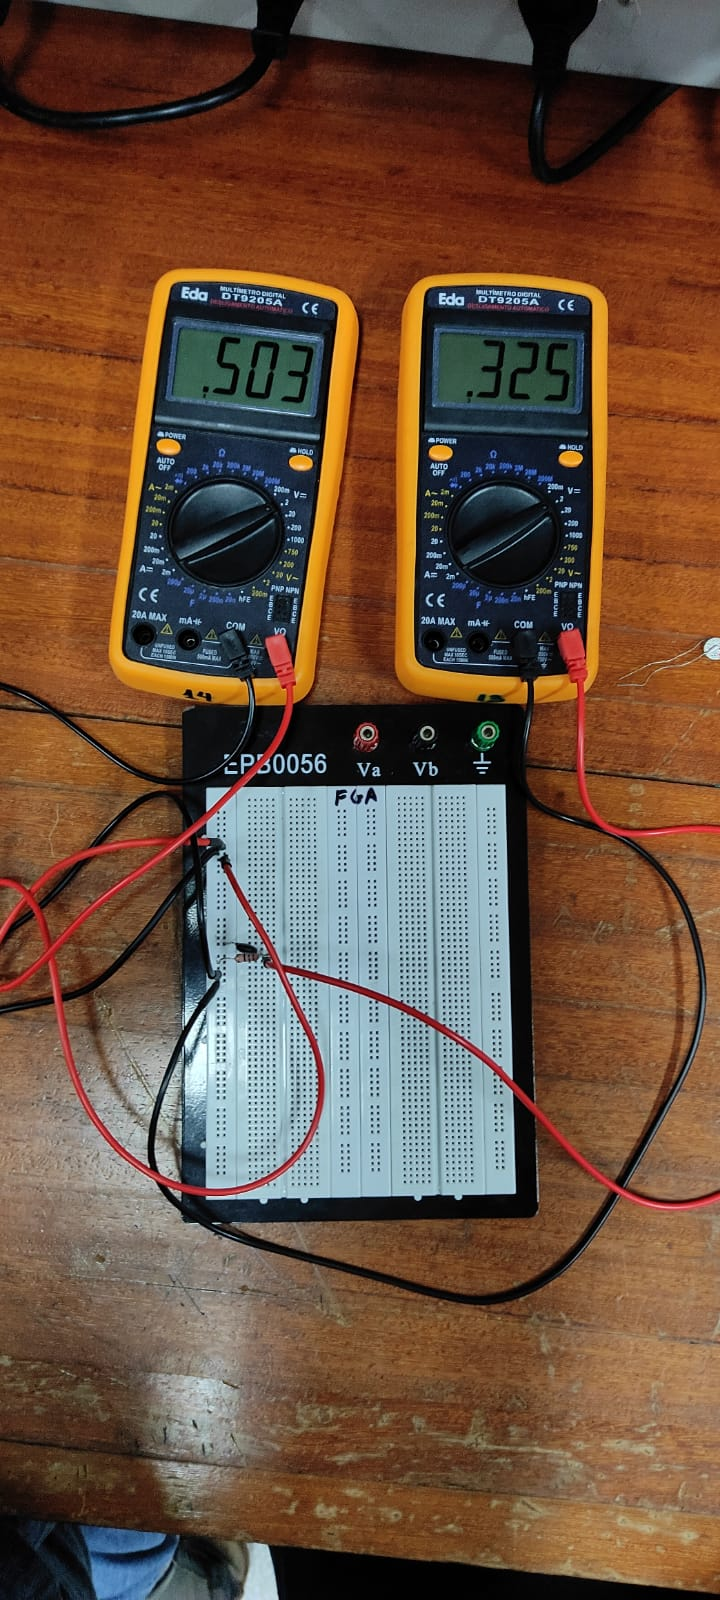
\includegraphics[trim={0 10cm 0 10cm}, clip, width=.9\textwidth]{0V5}
\caption{Circuito com alimentação de 0,5V.}
\end{subfigure}
\begin{subfigure}{.3\textwidth}
\centering
%\captionsetup{justification=centering,margin=1cm}
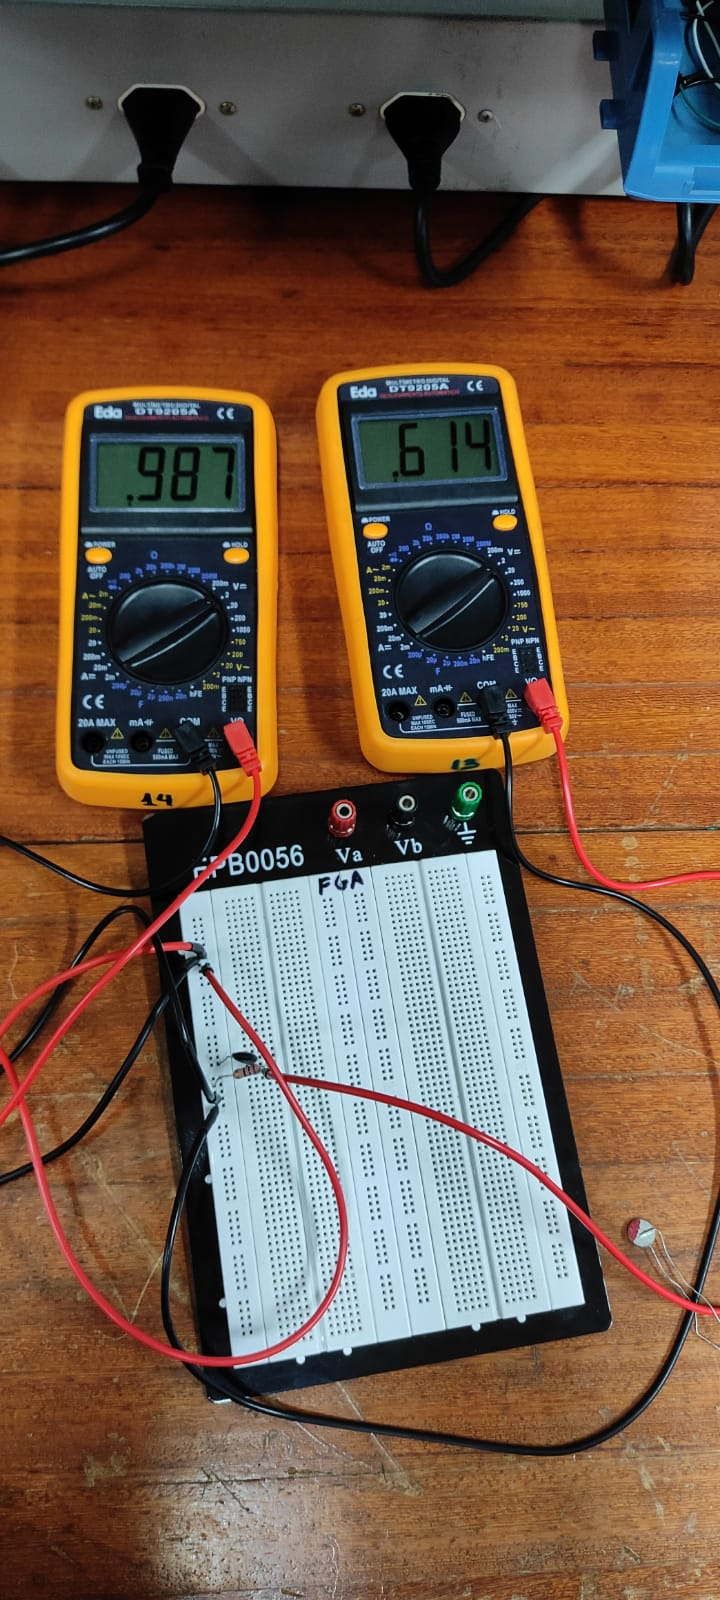
\includegraphics[trim={0 10cm 0 10cm}, clip, width=.9\textwidth]{1V}
\caption{Circuito com alimentação de 1,0V.}
\end{subfigure}
\begin{subfigure}{.3\textwidth}
\centering
%\captionsetup{justification=centering,margin=1cm}
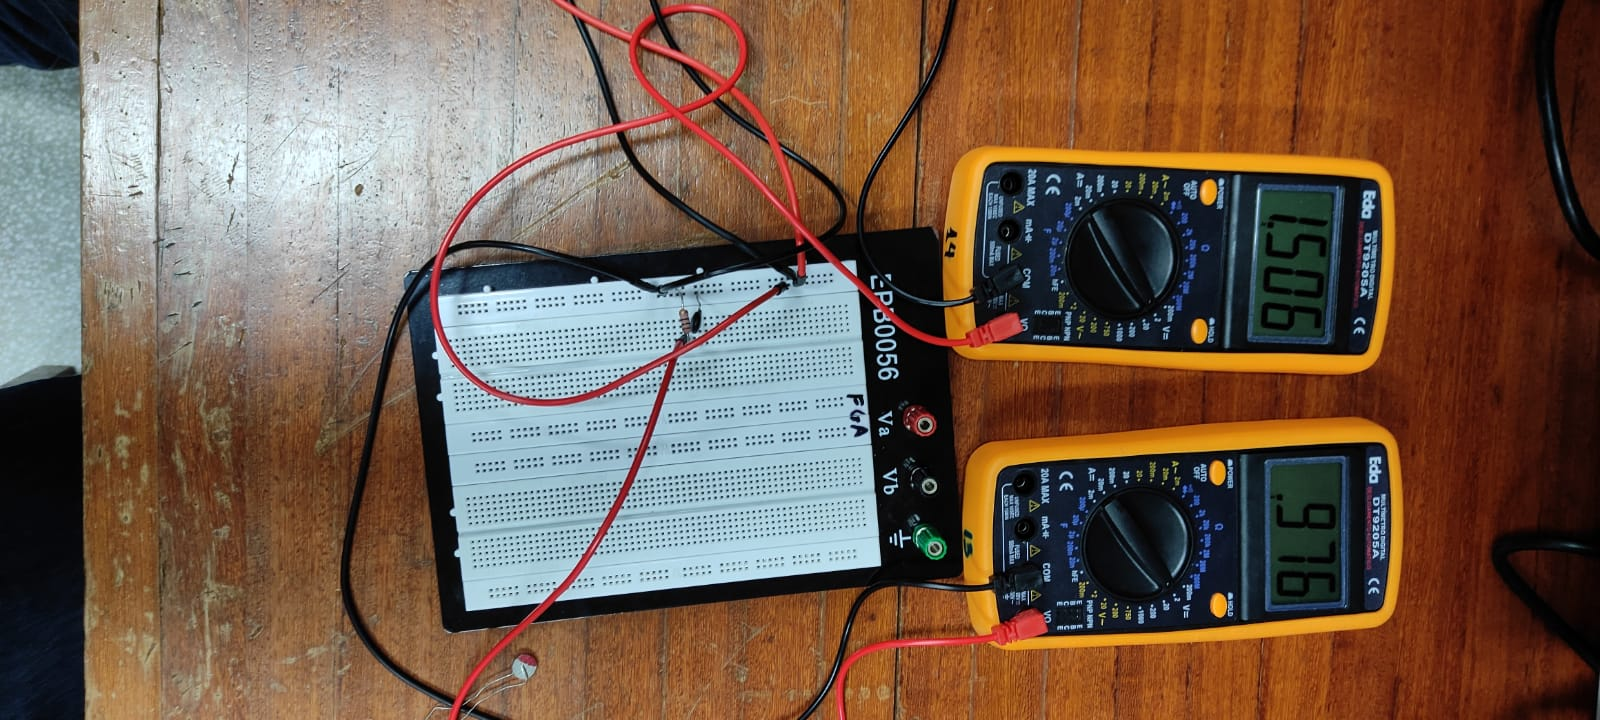
\includegraphics[trim={13cm 0cm 5cm 0cm}, clip, angle=90, width=.9\textwidth]{1V5}
\caption{Circuito com alimentação de 1,5V.}
\end{subfigure}
\begin{subfigure}{.3\textwidth}
\centering
%\captionsetup{justification=centering,margin=1cm}

\includegraphics[trim={0 10cm 5cm 15cm}, clip,width=.9\textwidth]{2V}
\caption{Circuito com alimentação de 2,0V.}
\end{subfigure}
\begin{subfigure}{.3\textwidth}
\centering
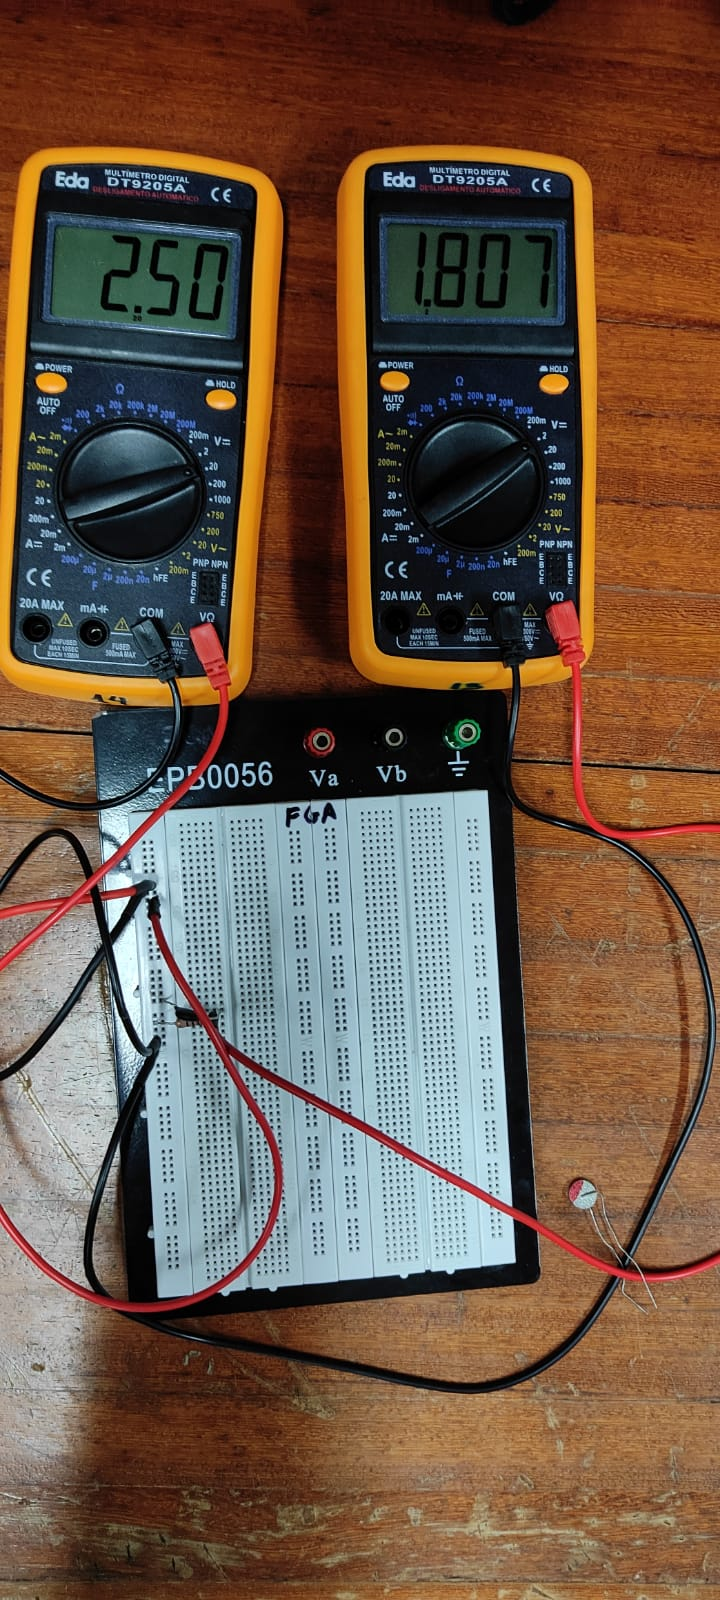
\includegraphics[trim={0 10cm 0 5cm}, clip, width=.9\textwidth]{2V5}
\caption{Circuito com alimentação de 2,5V.}
\end{subfigure}
\begin{subfigure}{.3\textwidth}
\centering
%\captionsetup{justification=centering,margin=1cm}
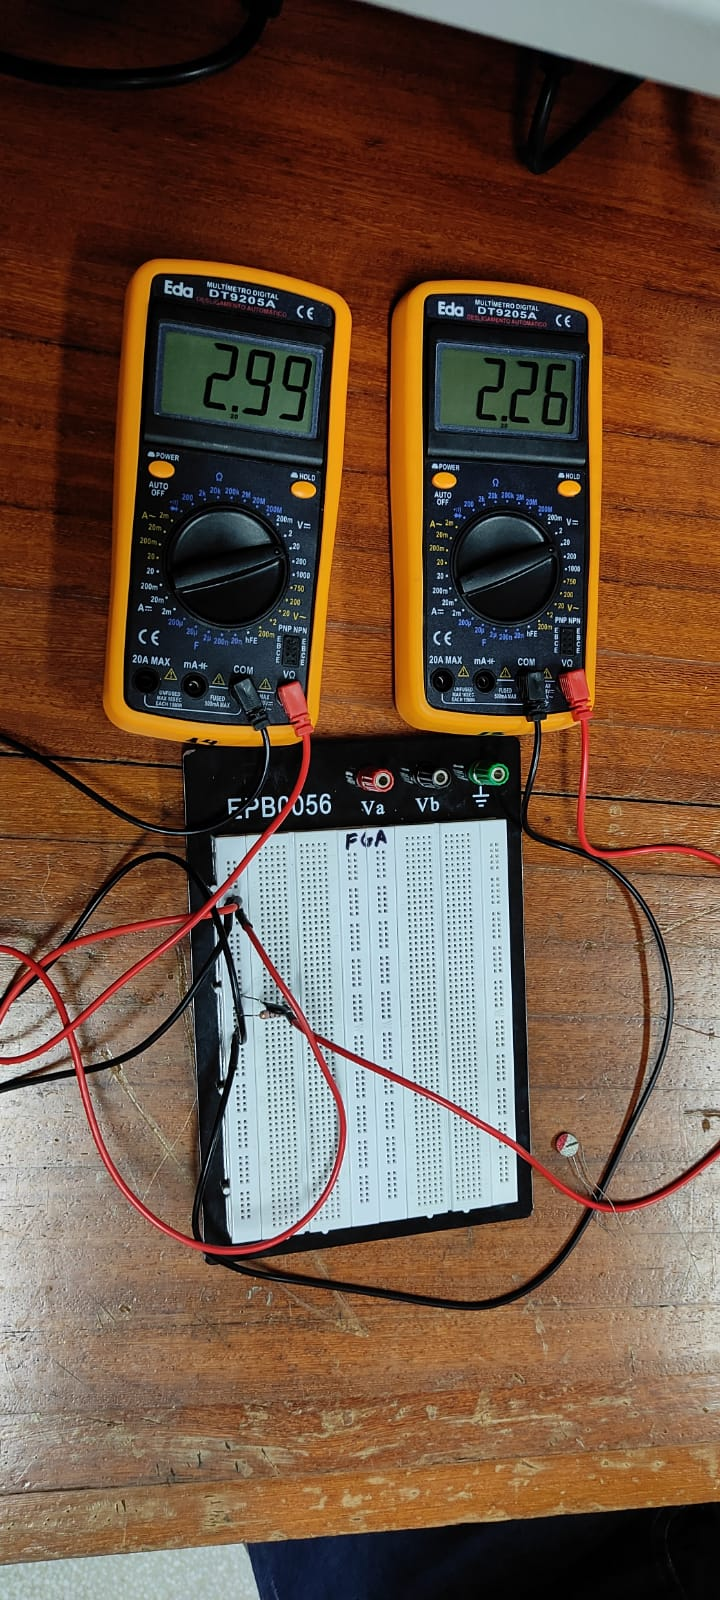
\includegraphics[trim={0 10cm 0 10cm}, clip, width=.9\textwidth]{3V}
\caption{Circuito com alimentação de 3,0V.}
\end{subfigure}
\begin{subfigure}{.3\textwidth}
\centering
%\captionsetup{justification=centering,margin=1cm}
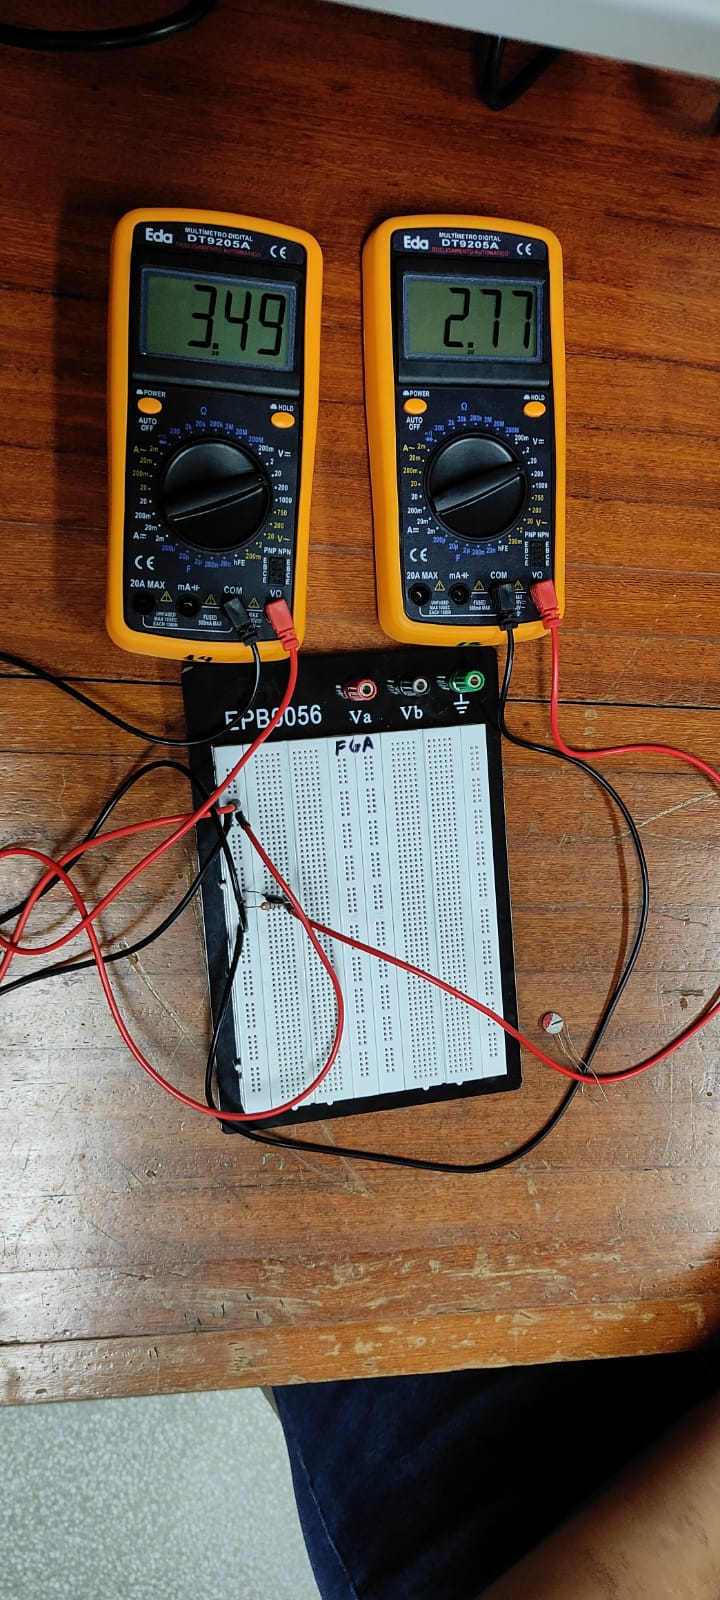
\includegraphics[trim={0 15cm 0 8cm}, clip, width=.9\textwidth]{3V5}
\caption{Circuito com alimentação de 3,5V.}
\end{subfigure}
\begin{subfigure}{.3\textwidth}
\centering
%\captionsetup{justification=centering,margin=1cm}

\includegraphics[trim={0 10cm 0 10cm}, clip, width=.9\textwidth]{4V}
\caption{Circuito com alimentação de 4,0V.}
\end{subfigure}
\caption{Medições realizadas com o circuito excitado.}
\label{fig:medicoes}
\end{figure}

A medição do resistor $R_2$ foi de $9,6\Omega$. Para tal medição, foi descontado
antes o valor da resistência das pontas de prova.

O gráfico da resistência em função da temperatura pode ser vista na figura 
\ref{fig:plot_temp}.


\begin{figure}[H]
  \centering
  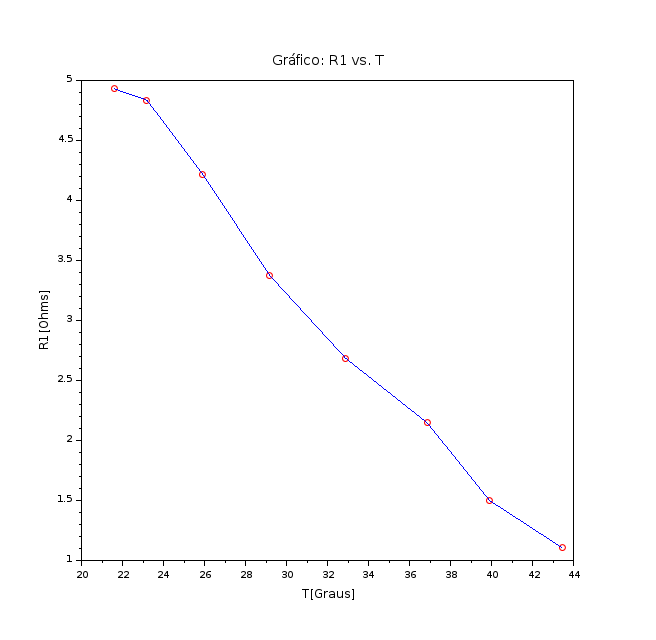
\includegraphics[width=.5\textwidth]{plot_temp}
  \caption{Gráfico da resistência em função da temperatura do componente.}
  \label{fig:plot_temp}
\end{figure}

\subsection{Ajuste do modelo de Steinhart-Hart a partir do método dos mínimos quadrados}

O ajuste do modelo de Steinhart-Hart pode ser ajustado pelo método dos mínimos quadrados. Tal ajuste pode ser visto pela figura \ref{fig:plot_steinhart}. A análise da adequação do modelo pode ser visot pelo erro quadrático médio, que para esse caso foi de $0,24$ fazendo o modelo adequado o ajuste pelo método dos mínimos quadrados. 

\begin{figure}[H]
  \centering
  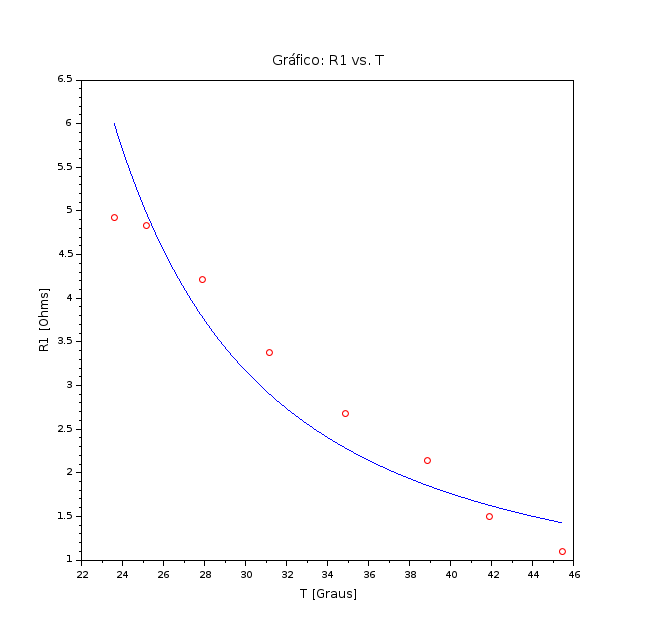
\includegraphics[width=.5\textwidth]{plot_steinhart}
  \caption{Gráfico da resistência R1 pela temperatura do modelo de Steinhart-Hart ajustado pelo método dos mínimos quadrados.}
  \label{fig:plot_steinhart}
\end{figure}



\subsection{Modelo de Steinhart-Hart a partir dos parâmetros fornecidos pelo fabricante. ($r_\infty, R_0, B$)}

Foi calculado a curva de modelo utilizando os parâmetros fornecidos pelo datasheet, como visto na figura \ref{fig:param_datasheet_steinhart}. Esse gráfico não apresentou acurácia tal qual o modelo ajustado pelo método dos mínimos quadrados por ser um valor de parâmetros geral, obtido sob condições controladas em meio a fábrica. Além disso, os dispositivos apresentam um desvio no processo de fabricação, fazendo que também haja interferência no resultado final.


\begin{figure}[H]
  \centering
  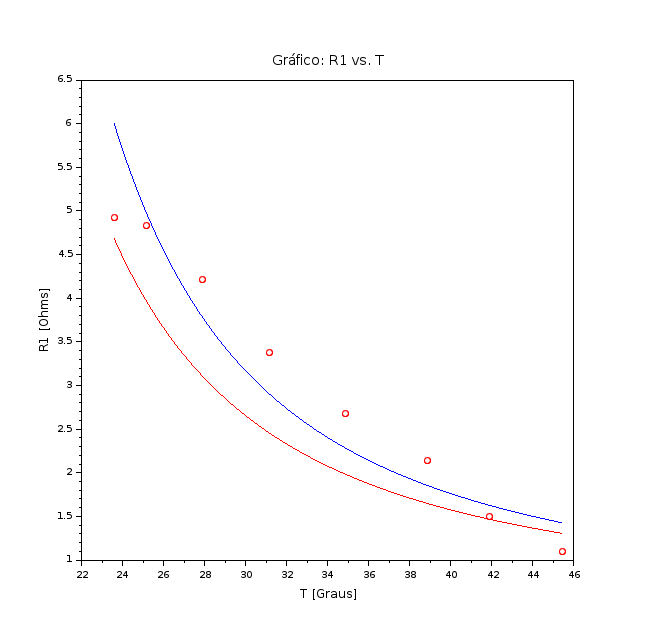
\includegraphics[width=.6\textwidth]{param_datasheet_steinhart}
  \caption{Modelo de Steinhart-Hart para obtenção da temperatura utilizando os parâmetros fornecidos pelo datasheet do componente.}
  \label{fig:param_datasheet_steinhart}
\end{figure}


\section{Questionário}

\subsection{Encontre 5 aplicações tecnológicas de termistores NTC e PTC. Cite as suas referências.}
\begin{itemize}

  \item Como um limitador de corrente inrush em circuitos de fonte de alimentação. Eles apresentam uma alta resistencia inicialimente o que previne altas correntes fluindo para o circuito quando este liga. Então, quando o circuito aquece, o termístor fica com baixa resistência, permitindo a passagem de correntes mais altas em operação normal. Estes termístores são normalmente muito maiores que os termístores utilizados para medição, e são propositalmente projetados para essa aplicação. Fonte: "http://www.ussensor.com/inrush-current-limiting-power-thermistors"
  \item Como sensores em aplicações automotivas para monitorar a temperatura de fluídos como a cabine de ar, ar externo, resfriamento do motor, temperatura do óleo do motor e alimentar o sistema de controle como a central de informação e o ECU. 
  \item Para monitorar a temperatura de uma incubadora. 
  \item Termístores são também comumente utilizados em termostátos digitais e para monitorar a temperatura de packs de baterias enquanto estão no processo de carregamento.
  \item Eles também são utilizados na mesa quente de impressoras 3D e também nos bicos de injeção, controlando o derretimento do filamento de plastico.
\end{itemize}


\subsection{Liste os vários tipos de materiais que são usados na fabricação de termistores NTC e PTC comerciais, citando as suas fontes, e relatando: i) Composição do material usado; ii) Mecanismo físicico de sensibilidade à temperatura.}


Termístores NTC são fabricados a partir de óxidos do grupo de metais ferro, tais como: Cromo (CrO), mangânes(MnO), cobalto (CoO), ferro (óxidos de ferro), e níquel (NiO).

 PTCs são normalmente feitos a partir de bário (Ba), estrôncio, ou titanetes de chumbo.


Os NTCs funcionam a partir de um princípio muito simples: com a subida de temperatura, o número de portadores de carga ativa são promovidos para a banda de produção. Quanto mais cargas estão disponíves, mais corrente o material pode conduzir. 


Os PTC são em maioria feitos a partir de cerâmica de porlicristalina dopada que tem uma propriedade que sua resistência cresce abruptamente em uma certa temperatura crítica. Já o barium titaneto é um material ferroelétrico e sua constante dielétrica varia com a temperatura. Abaixo do ponto de temperatura de Cure, a alta constante dielétrica privine a formação de uma barreira potência enetr os grãos de cirstal, conduzindo a uma baixa resistencia. Nessa região o dispositivo tem um coeficiente de temperatura negativo baixo. No ponto da temperatura de Courie, a constante dielétrica decaí suficientemente para permitir a formação de uma barreira potencial para os limites dos grãos, e a resistência aumenta fortemente com a temperatura. Para temperatura mais altas, o material se converte em um comportamento característico de um NTC.

Fonte:  Morris, Alan S. (2020). "Chapter 14 - Temperature measurement". Measurement and instrumentation theory and application. Reza Langari (Third ed.). Amsterdam. ISBN 978-0-12-817142-4. OCLC 1196195913.


\end{document}
